\newpage
\section{Simulation Analysis}
\label{sec:simulation}


\subsection{Bandpass filter}

This type of filter, with the characteristics that were mentioned in the Introduction, has several applications:

\begin{itemize}
    \item BPFs (Bandpass filters) are extensively used in wireless transmitters and receivers. The main function of this filter in a transmitter is to limit the bandwidth of the o/p signal to the band allotted for the transmission. This avoids the transmitter from interfering with further stations.
    \item In a receiver, a Band-Pass filter allows signals within a selected range of frequencies to be heard or decoded, while preventing signals at unwanted frequencies from getting through.
    \item A Band-Pass filter also optimizes the signal-to-noise ratio and sensitivity of a receiver.
    This filters are used in all types of instruments as well as in Sonar, Seismology and even medical applications like EEGs and Electrocardiograms. These filters are also extensively used in optics like lasers, LIDARS, etc.
    \item A BPF (Band-Pass Filter) permits an exact frequency range to pass, while blocking frequencies that are lower and higher. A good application is in Audio Signal Processing, where a particular range of frequencies of sound is required while removing the rest.
    \item   Band-Pass filters are used in communication systems for selecting a specific signal from a range of signals.
\end{itemize}


\subsection{Implementation}

The first implementation consisted in an High-Pass filter at the input of the OPAMP, an OPAMP with negative feedback, so that the gain was 100, and a Low-Pass filter at the output. In this way we were able to obtain the Band-Pass filter with the desired gain. 

After this first implementation, we realized that the OPAMP itself, due to the components it contained, cut the high frequencies. In this way, we removed the low pass filter at the OPAMP output, because of the components redundancy and to reduce the cost.


The implemented circuit and the values of its components are shown in the figure and tables below:

\begin{figure}[H] \centering
\includegraphics[scale=0.3]{t5_circuit.pdf}
\caption{Band-Pass Filter circuit}
\label{fig:t5}
\end{figure}

\begin{table}[H]
  \centering
  \begin{tabular}{|l|r|}
    \hline    
    {\bf Name} & {\bf Value [k$\Omega$] or [uF]} \\ \hline
    R1 &  1\\ \hline
R2 &  1\\ \hline
R3 &  1\\ \hline
C1 &  220\\ \hline
C2 &  220\\ \hline
C3 &  220\\ \hline

  \end{tabular}
  \caption{Values of the components}
  \label{tab:www}
\end{table}
\vspace{-0.2in}

\subsection{Frequency Response}

After the circuit implementation, its behaviour was analyzed as a frequency function. As we expected, the circuit behaves like a Band-Pass filter with a center frequency of approximately 1kHz and a gain of 100. 

The graphs below show the magnitude and phase response in relation to the frequency:



\begin{figure}[H] \centering
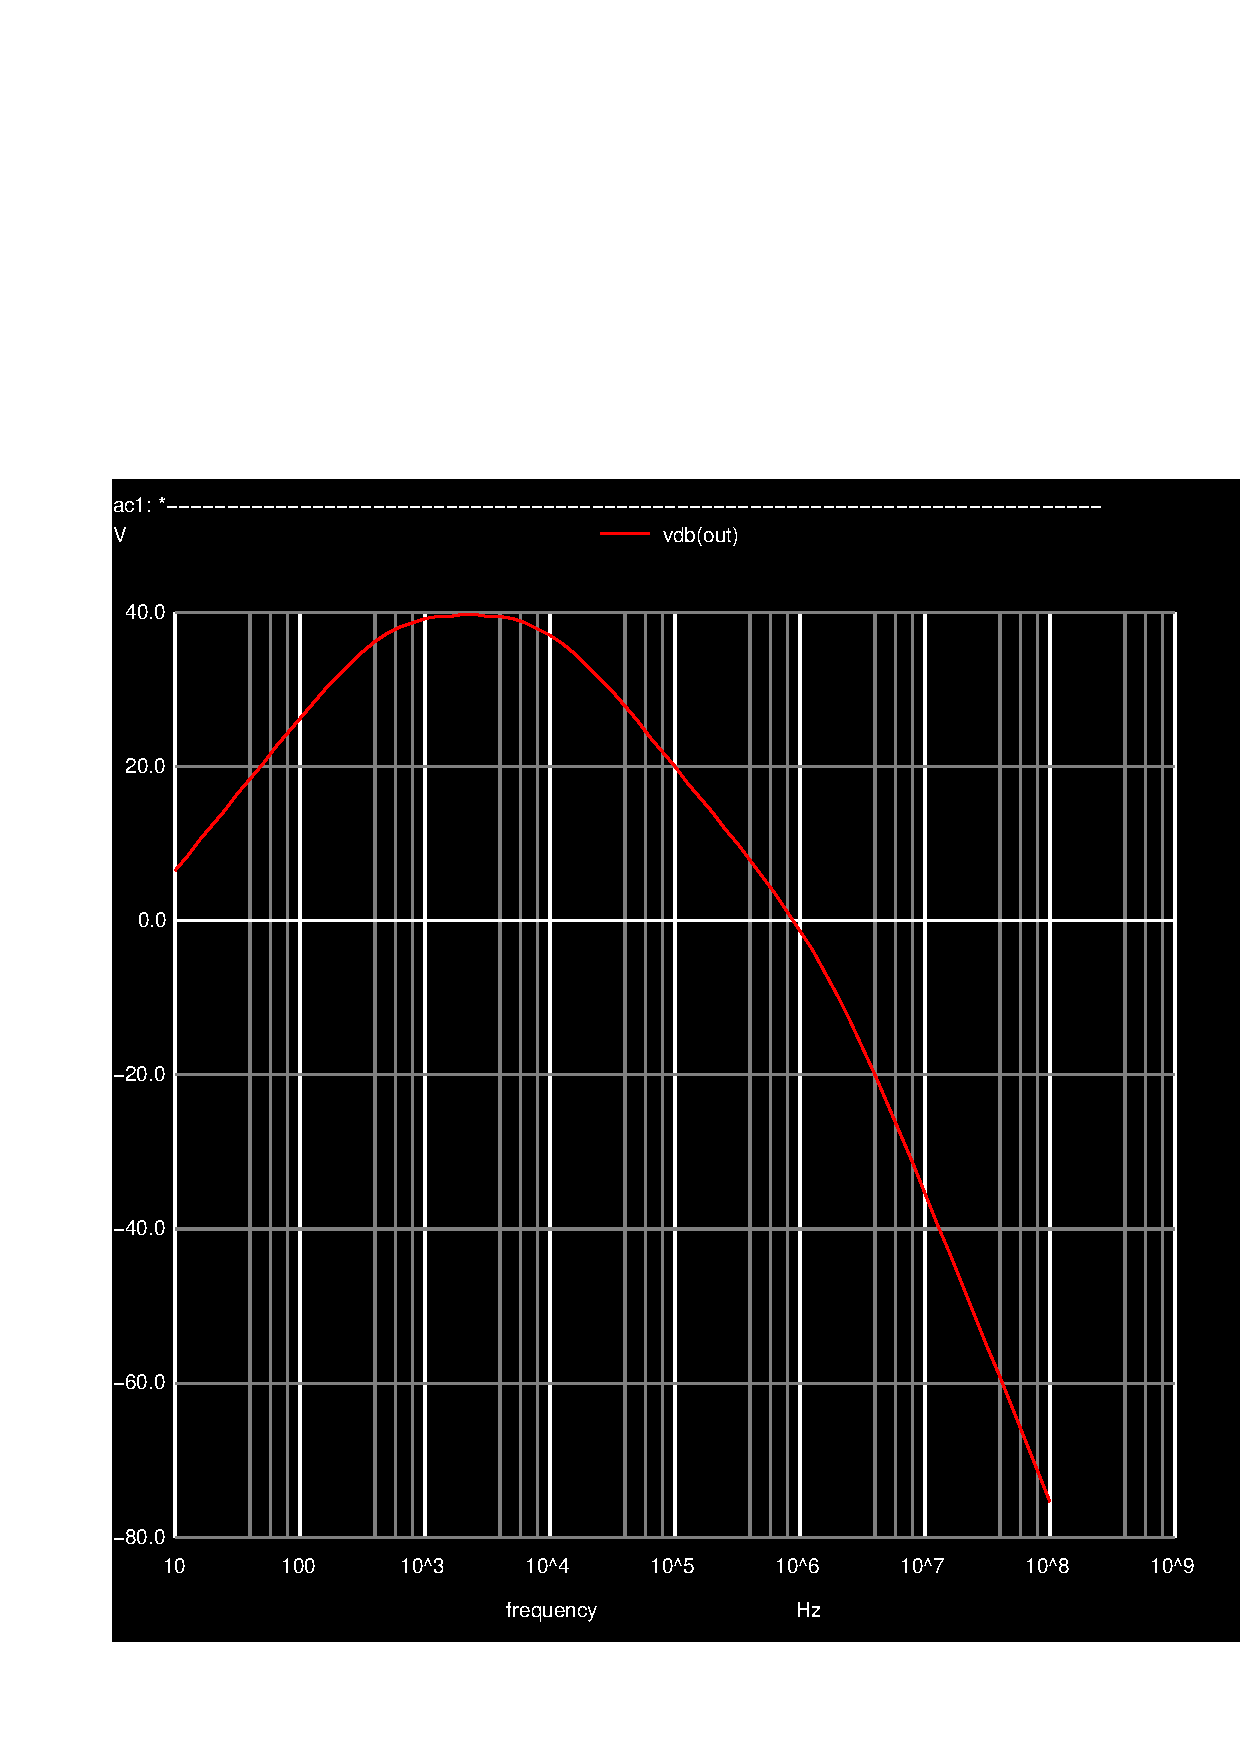
\includegraphics[scale=0.28]{vo1db.pdf}
\caption{Magnitude frequency response}
\label{fig:t511}
\end{figure}

\vspace{-0.8in}



\begin{figure}[H] \centering
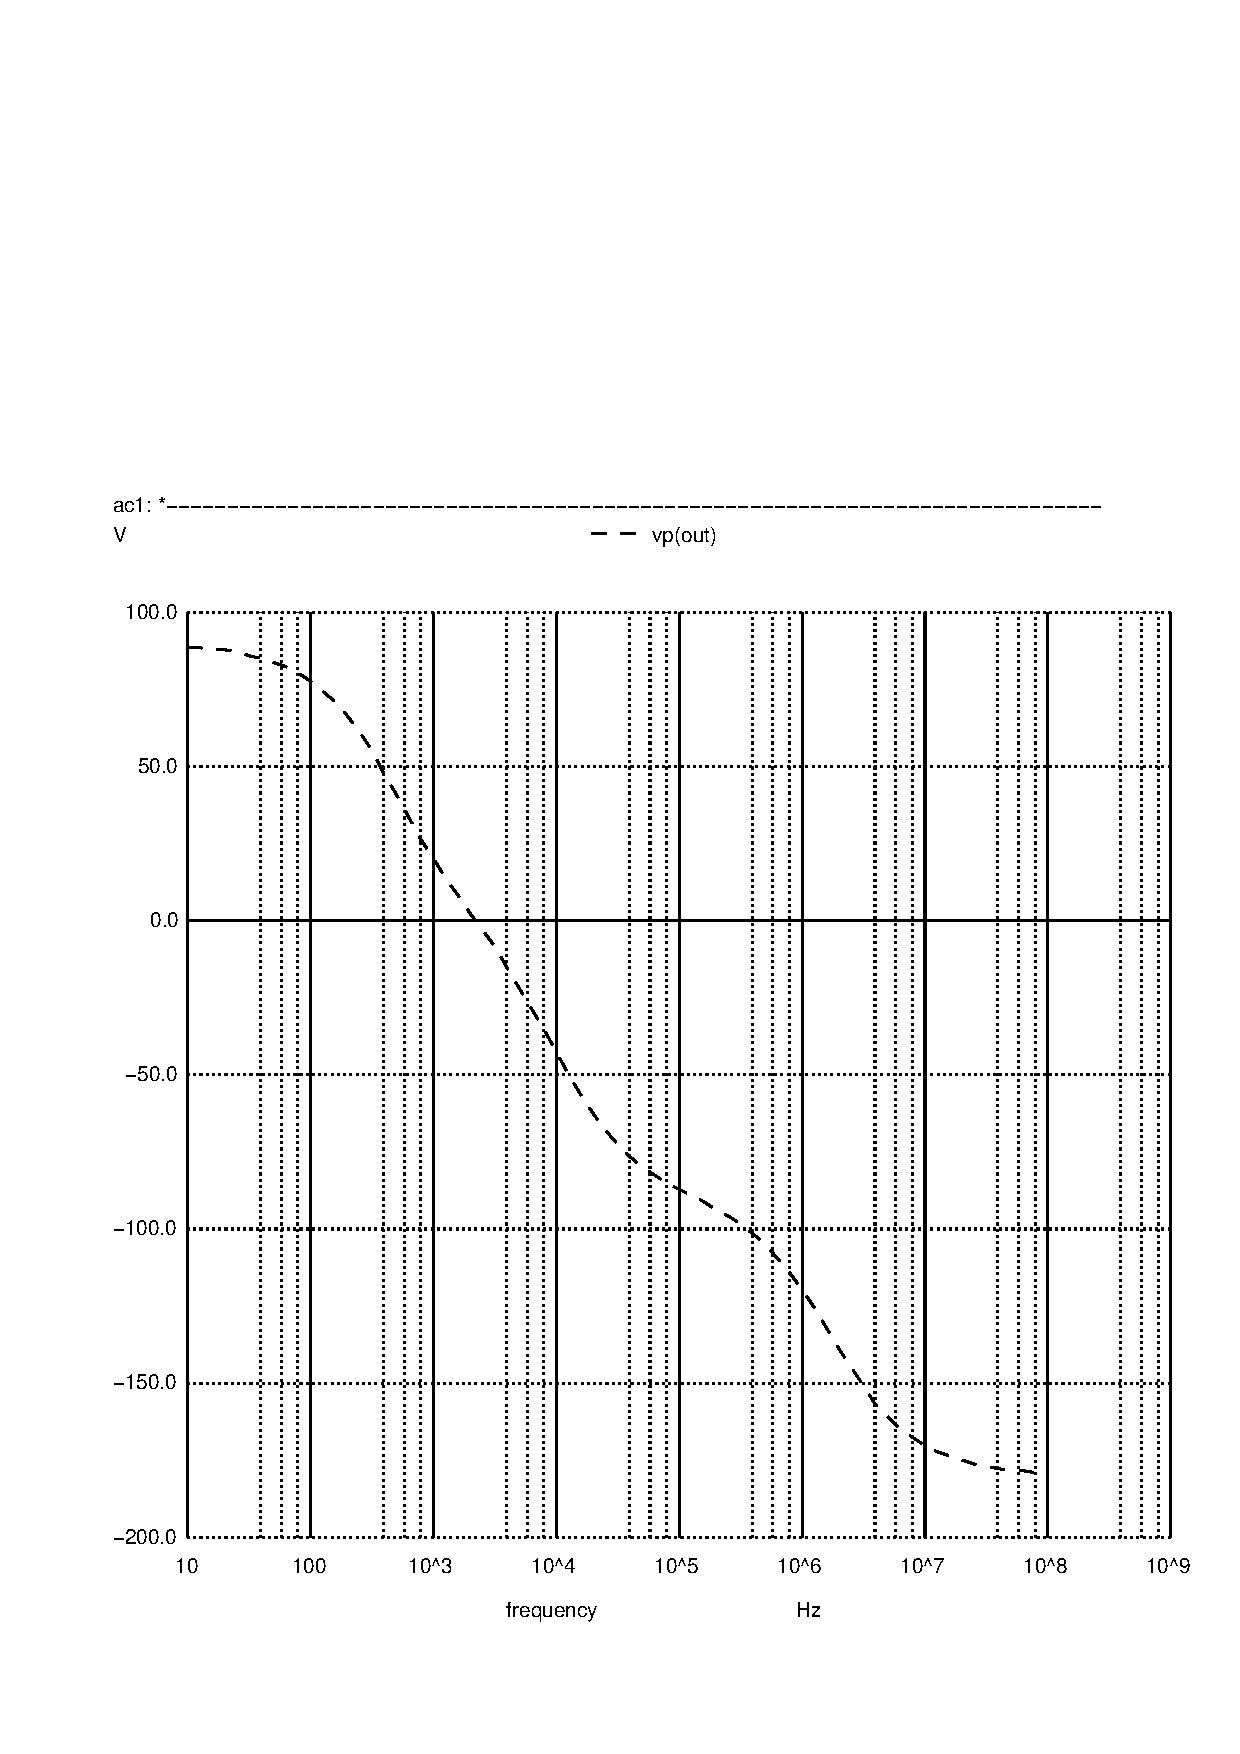
\includegraphics[scale=0.28]{vo1f.pdf}
\caption{Phase frequency response}
\label{fig:t52}
\end{figure}

\subsection{Voltage gain deviation}

One of the requirements of the implementation was that at the frequency of 1000Hz, the gain should be 400dB, which means that the ratio between the output and input signal was 100. To measure this value in the simulation, the measure function was used to analyse the frequencies. The results are shown in table 2: 

\begin{table}[H]
  \centering
  \begin{tabular}{|l|r|}
    \hline    
    {\bf Name} & {\bf Value [dB] or non-dimensional} \\ \hline
    centralgain & 9.763641e+01\\ \hline
centralgaindb & 3.979224e+01\\ \hline

  \end{tabular}
  \caption{Values of Gain}
  \label{tab:r}
\end{table}

As can be seen the value of our gain is very close to 100, that was the objective.


\subsection{Central Frequency Deviation}

The second requirement was that the central frequency was 1kHz. To determine this central frequency, we proceeded to measure the lower and upper frequencies where the gain dropped 3dB from its maximum. Subsequently, the central deviation frequency was computed from a geometric mean, that is, the root of the product of the upper and lower frequencies. In the following tables, we present the results that we have obtained.

\begin{table}[H]
  \centering
  \begin{tabular}{|l|r|}
    \hline    
    {\bf Name} & {\bf Value [Hz] } \\ \hline
    freqlow & 9.456061e+01\\ \hline
freqhigh & 1.056765e+04\\ \hline
centralfreq & 9.996417e+02\\ \hline

  \end{tabular}
  \caption{Values of Gain}
  \label{tab:r}
\end{table}


\subsection{Input and Output impedance}

These two parameters are very important to predict the behavior of the implemented circuit.
At the frequency we are working on, we want the input impedance to be as high as possible, and the output impedance as low as possible so that there is no signal degradation when we implement it in other circuits. 

\subsubsection{Input impedance}

To determine the input impedance it was necessary to place a very large Load ($Z_L=\infty$) and remove the components upstream of the OPAMP, C1 and R1. After placing this load at the output of the circuit, the $v_I$, $v_-$ and the current entering the non-inverting input were measured. The calculation was done with the following expression: 

\begin{equation}
    Z_L= \left. \frac{v_I}{i_I} \right|_{Z_i=\infty}
\end{equation}

The obtained value is adequate to the intended one, however it doesn't fit reference interval.(1-10M $\Omega$)

\begin{table}[H]
  \centering
  \begin{tabular}{|l|r|}
    \hline    
    {\bf Name} & {\bf Value $[M\Omega]$ } \\ \hline
    zinput & 5.121429e+02\\ \hline

  \end{tabular}
  \caption{Value of Zi}
  \label{tab:r}
\end{table}

We also made the input impedance plot (Figure~\ref{fig:zi}) to verify the behavior. As noted, the input impedance value does not change much with frequency. 
\vspace{-2 cm}
\begin{figure}[H]
    \centering
    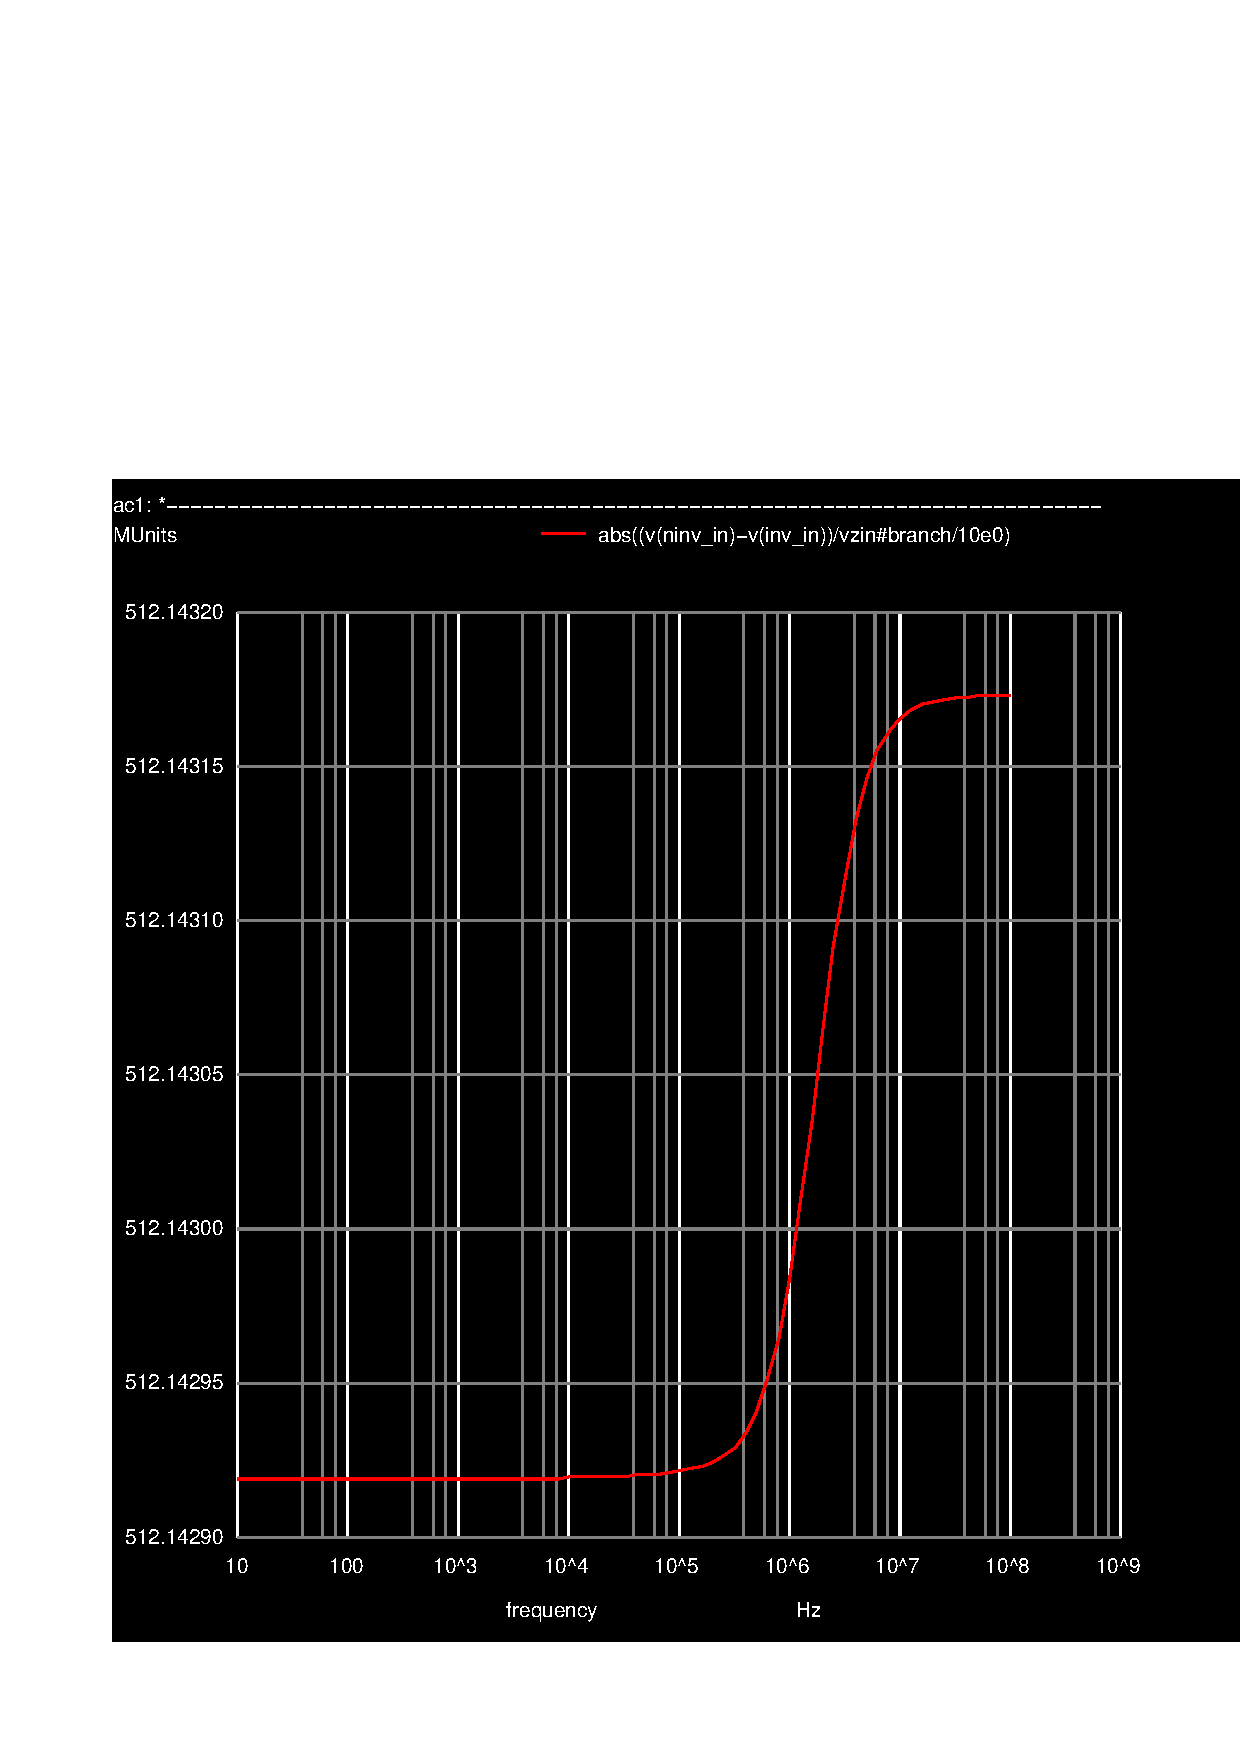
\includegraphics[scale=0.55]{z_i.pdf} 
    \caption{Frequency response of input impedance}
    \label{fig:zi}
\end{figure}

\subsubsection{Output impedance}

To determine the input impedance it was necessary to implement a slightly different circuit. The signal source was placed at the OPAMP output, and the current and voltage at the OPAMP output were measured, from its ratio, the output impedance was determined.

\begin{equation}
    Z_O = \left. \frac{v_O}{i_O} \right|_{v_i=0} 
\end{equation}

The obtained value is again adequate to the intended one, and is slightly lower than the reference values of the OPAMP (10-100 $\Omega$).

\begin{table}[H]
  \centering
  \begin{tabular}{|l|r|}
    \hline    
    {\bf Name} & {\bf Value $[\omega]$ } \\ \hline
    zoutput & 5.038865e+00\\ \hline

  \end{tabular}
  \caption{Value of $Z_O$}
  \label{tab:r}
\end{table}

We also made the output impedance plot (Figure~\ref{fig:zo}) to verify its behavior. As we noted, the output impedance, after reaching values close to 10kHz, increases substantially.

\vspace{-1.5in}
\begin{figure}[H] \centering
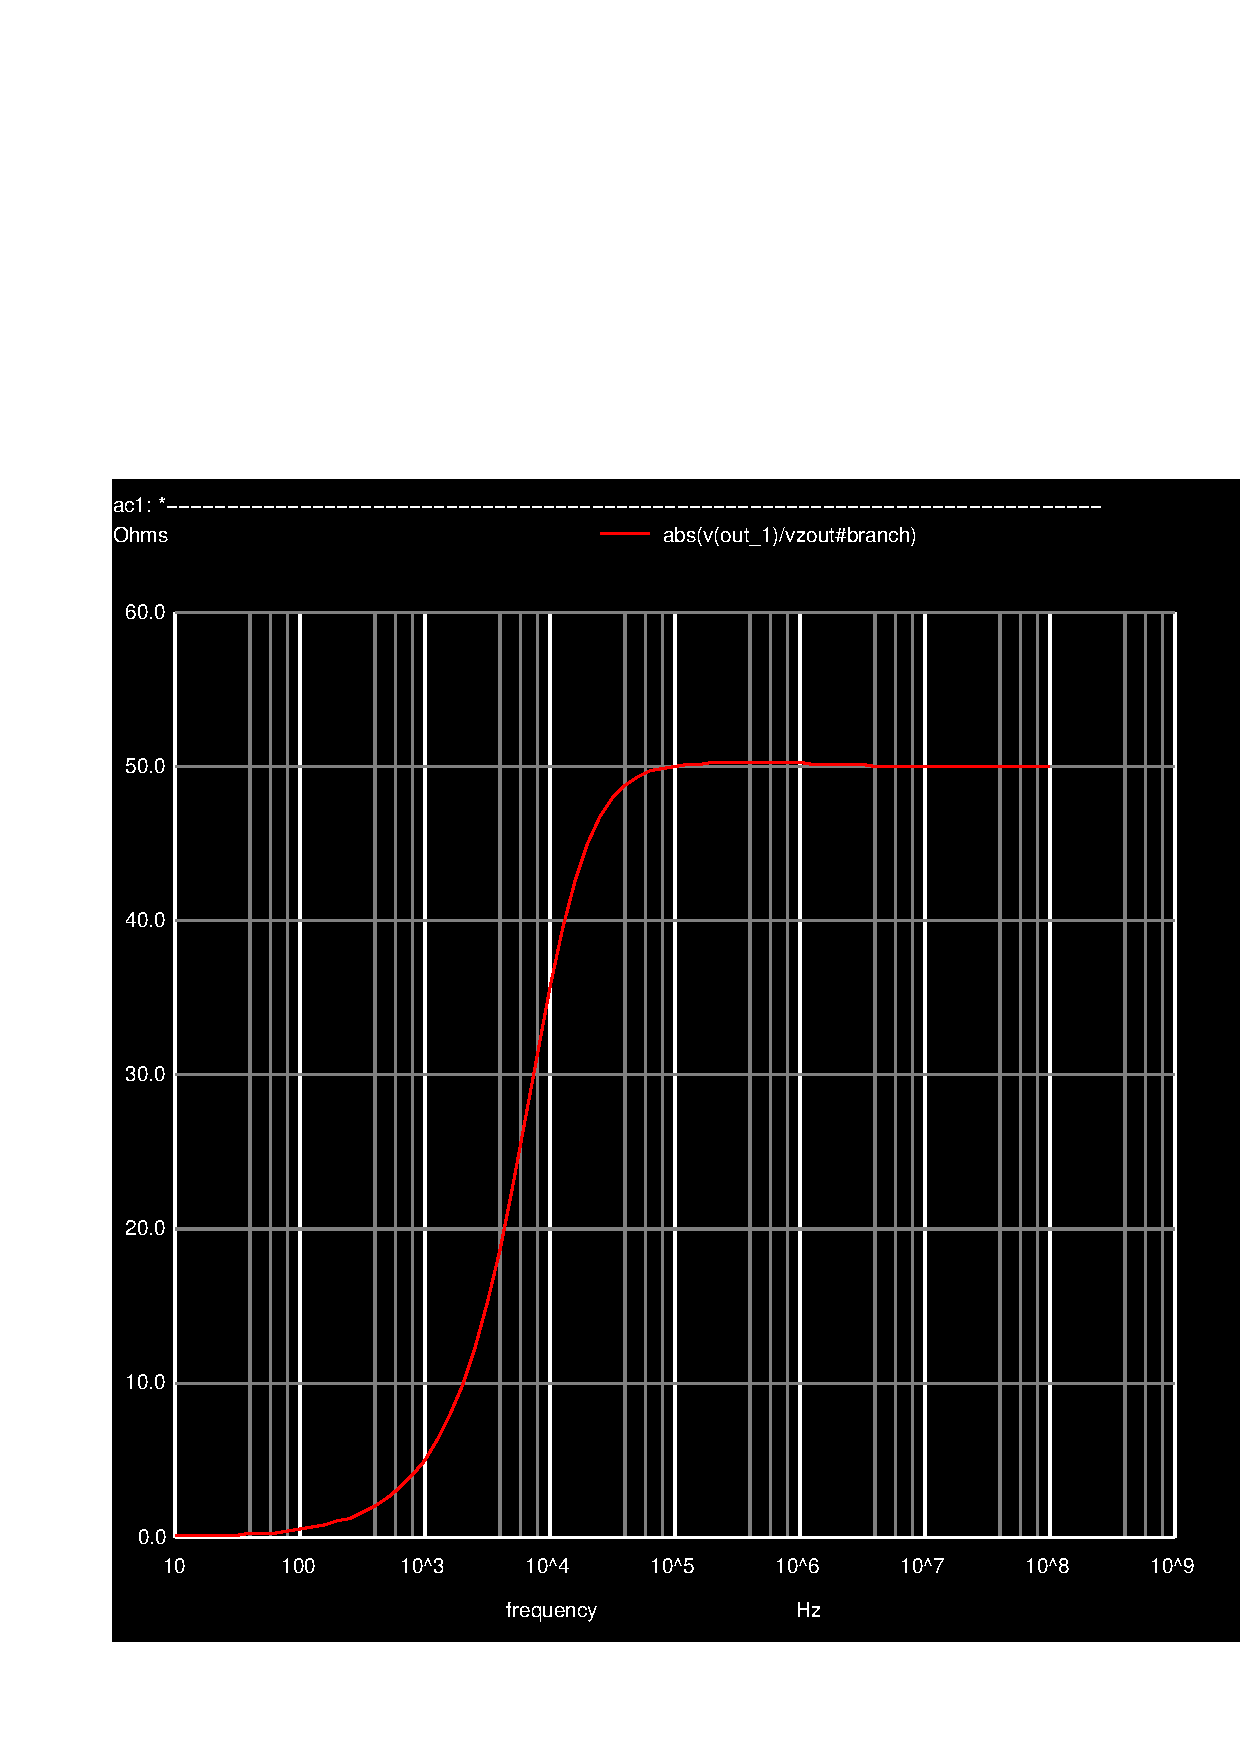
\includegraphics[scale=0.55]{z_o.pdf}
\caption{Frequency response of output impedance}
\label{fig:zo}
\end{figure}

